\documentclass{article}
\usepackage{graphicx}
\graphicspath{ {./plots/} }

\title{Berekeley CS 294-112: Deep Reinforcement Learning Homework 1}
\author{John Dang}
\date{}

\begin{document}
\maketitle
    \section{Behavioral Cloning (Imitation Learning)}
    Imitation learning was implemented using a vanilla 
    feed-forward neural network with 4 hidden layers with 
    512,256,128, and 64 hidden units respetively and ReLU 
    activations for all layers except output. The network takes 
    observations as vectors and outputs actions. The dimensions of 
    the input and output vectors are determined by the task.
    During training the network received a dataset of 10 rollouts for each 
    task and was training for 50 epochs with a batch size of 128 observations. 
    The policy was evaluated on 5 newly sampled episodes following each training 
    epoch. Imitation learning performed well for tasks including Ant-v2 and HalfCheetah-v2 and
    performed poorly for the Humanoid-v2 task where performance from the learned 
    policy was much worse than the expert.\\

    \begin{tabular}{ |p{3cm}||p{1.5cm}|p{1.5cm}|p{1.5cm}|p{1.5cm}| }
        \hline
        \multicolumn{5}{|c|}{\textbf{Imitation, and Expert Policy Reward Comparison}} \\
        \hline
        & \multicolumn{2}{|c|}{\textbf{Imitation}}  & \multicolumn{2}{|c|}{\textbf{Expert}} \\
        \cline{2-5}
        & \textbf{Mean} & \textbf{STD} & \textbf{Mean} & \textbf{STD} \\
        \hline
        \textbf{Ant-v2}         & 4633.421    & 56.376      & 4838.639      & 89.365 \\
        \hline
        \textbf{HalfCheetah-v2} & 4058.767    & 66.907      & 4177.480      & 97.426 \\
        \hline
        \textbf{Hopper-v2}      & 1694.749    & 308.172     & 3779.356      & 2.931 \\
        \hline
        \textbf{Humanoid-v2}    & 346.837     & 52.922      & 10403.923     & 53.300 \\
        \hline
        \textbf{Reacher-v2}     & -6.1001     & 2.428       & -4.470        & 1.591 \\
        \hline
        \textbf{Walker2d-v2}    & 4481.929    &656.555      & 5512.973      & 48.089\\
        \hline
    \end{tabular}

    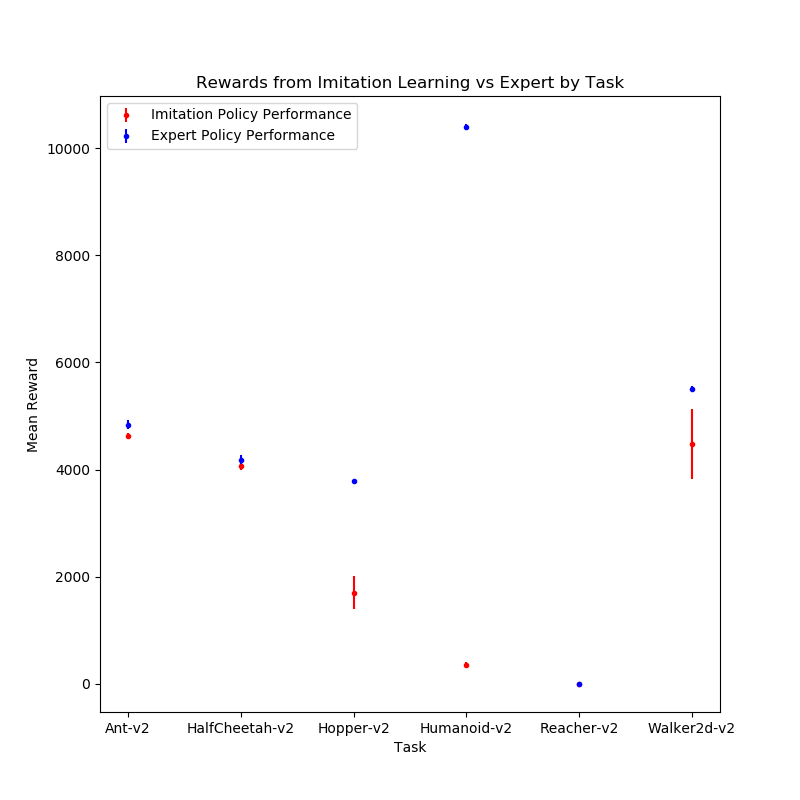
\includegraphics[scale=0.7]{imitationExpertComparison}\\

    As the number of training epochs increases, average reward achieved by 
    the policy increases, as expected in a traditional supervised learning 
    setting. On tasks where imitation learning performs comparibly to the 
    expert, performance increases rapidly with epochs and plateaus at expert performace.
    For other tasks, improvement is slower as shown in the learning curves below.

    \noindent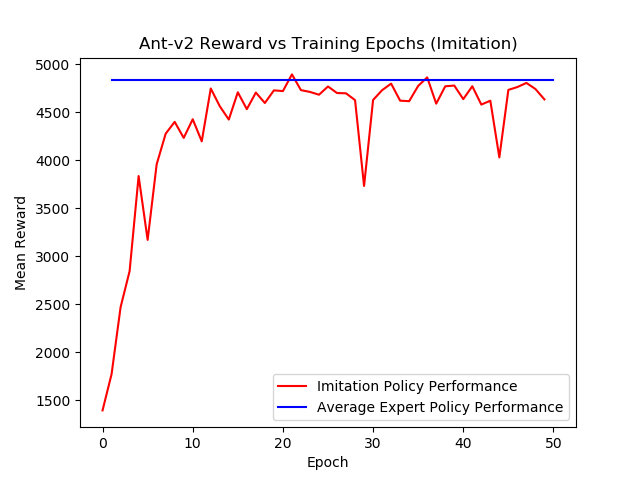
\includegraphics[scale=0.4]{Ant-v2Imitation} 
    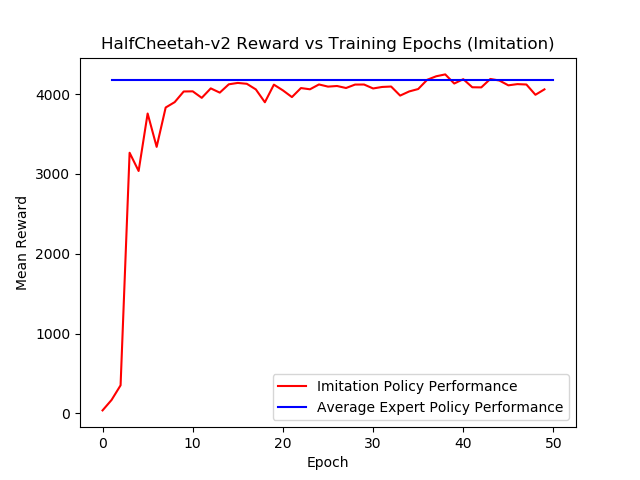
\includegraphics[scale=0.4]{HalfCheetah-v2Imitation}\\
    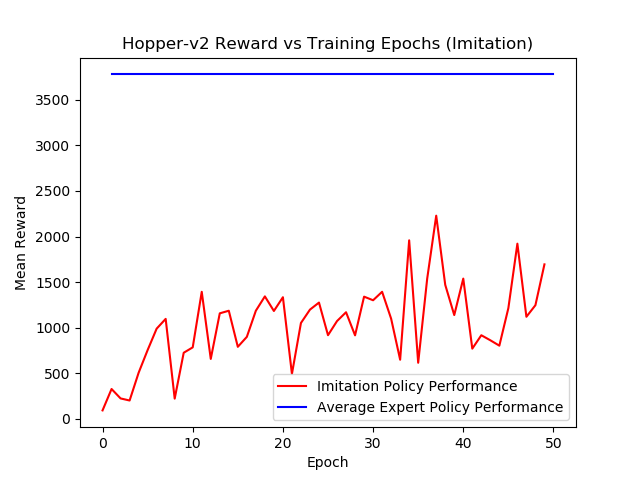
\includegraphics[scale=0.4]{Hopper-v2Imitation}
    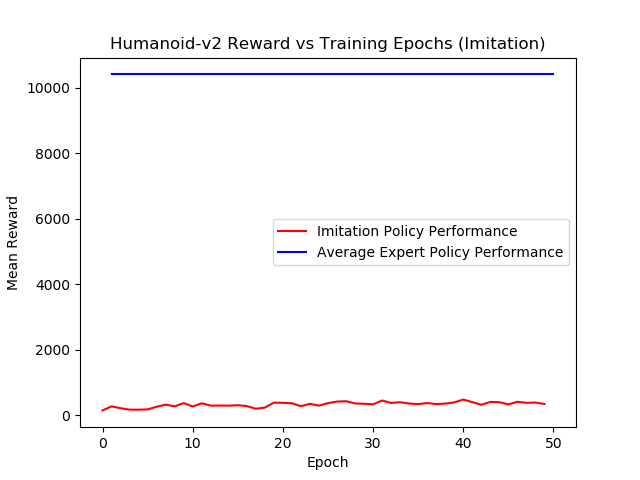
\includegraphics[scale=0.4]{Humanoid-v2Imitation}\\
    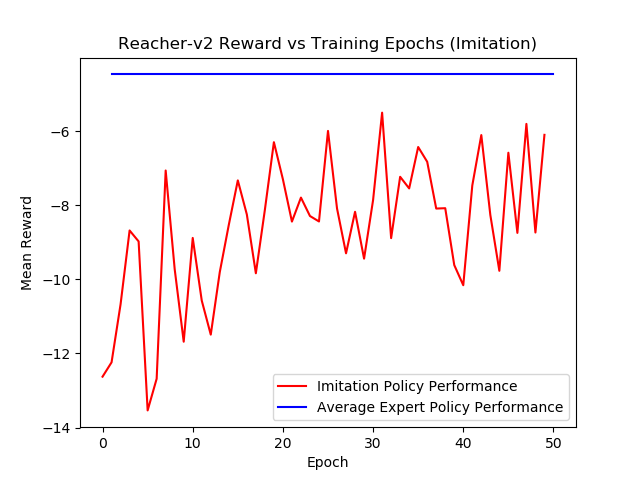
\includegraphics[scale=0.4]{Reacher-v2Imitation}
    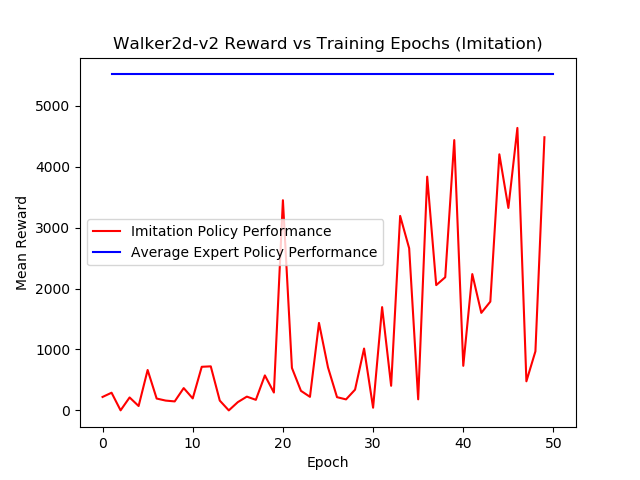
\includegraphics[scale=0.4]{Walker2d-v2Imitation}\\

    \pagebreak

    \section{Dataset Aggregation (Dagger)}
    Dagger was implemented using the same neural network architecture 
    mentioned above for imitation learning. The same imitation learning 
    procedure detailed above for imitation is performed before 20 dagger loops for 
    each task. Within each dagger loop, 5 new rollouts are performed using the 
    learned policy and labeled by the expert for aggregation with the original 
    dataset. As expected, using Dagger allows for learning of a policy significantly 
    closer in performance to that of the expert policy in all tasks. For 
    Humanoid-v2, Dagger achieves comparable performance to the expert, where imitation
    learning did not. Dagger achieves performance improvement over 
    pure imitation learning on all tasks including those where imitation learning was already 
    comparable to the expert policy performance.\\

    \noindent\begin{tabular}{ |p{3cm}||p{1.5cm}|p{1.5cm}|p{1.5cm}|p{1.5cm}|p{1.5cm}|p{1.5cm}| }
        \hline
        \multicolumn{7}{|c|}{\textbf{Imitation, Dagger, and Expert Policy Reward Comparison}} \\
        \hline
        & \multicolumn{2}{|c|}{\textbf{Imitation}} & \multicolumn{2}{|c|}{\textbf{Dagger}} & \multicolumn{2}{|c|}{\textbf{Expert}} \\
        \cline{2-7}
        & \textbf{Mean} & \textbf{STD} & \textbf{Mean} & \textbf{STD} & \textbf{Mean} & \textbf{STD} \\
        \hline
        \textbf{Ant-v2}         & 4633.421    & 56.376      & 4771.465      & 127.483       & 4838.639      & 89.365 \\
        \hline
        \textbf{HalfCheetah-v2} & 4058.767    & 66.907      & 4189.402      & 40.374        & 4177.480      & 97.426 \\
        \hline
        \textbf{Hopper-v2}      & 1694.749    & 308.172     & 3778.243      & 2.105         & 3779.356      & 2.931 \\
        \hline
        \textbf{Humanoid-v2}    & 346.837     & 52.922      & 8313.896      & 3884.014      & 10403.923     & 53.300 \\
        \hline
        \textbf{Reacher-v2}     & -6.1001     & 2.428       & -3.138        & 1.701         & -4.470        & 1.591 \\
        \hline
        \textbf{Walker2d-v2}    & 4481.929    &656.555      & 5507.156      & 71.321        & 5512.973      & 48.089\\
        \hline
    \end{tabular}

    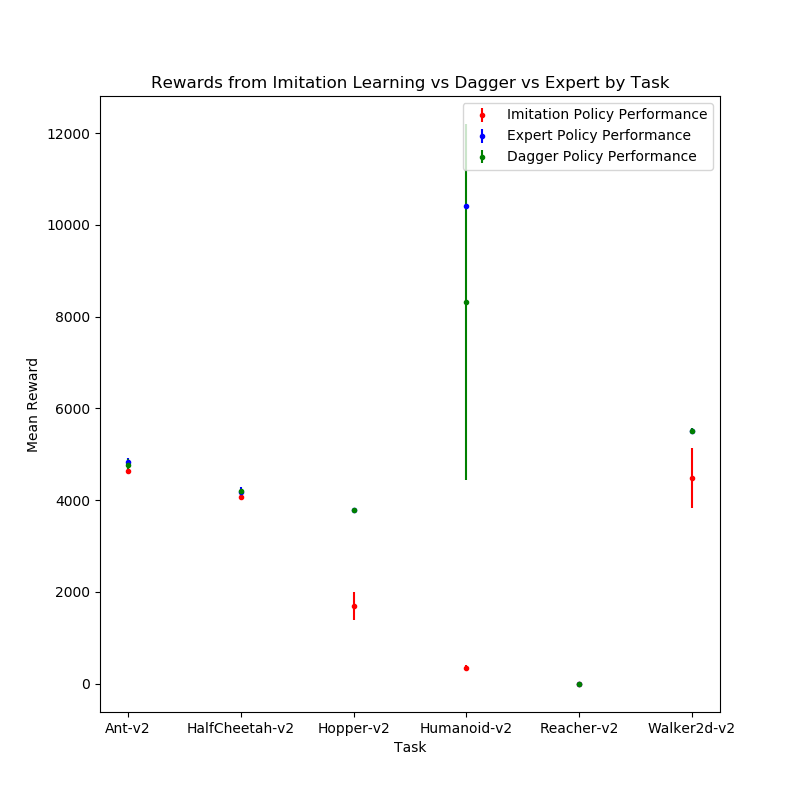
\includegraphics[scale=0.7]{overallComparison}\\
    
    Dagger performance increases with the number of Dagger loops. Performance 
    improves until reaching expert level performance, where the learning 
    curve begins to plateau.


    \noindent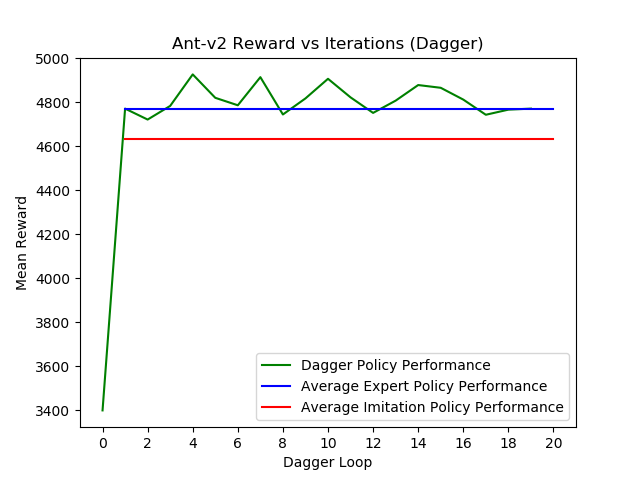
\includegraphics[scale=0.4]{Ant-v2Dagger}
    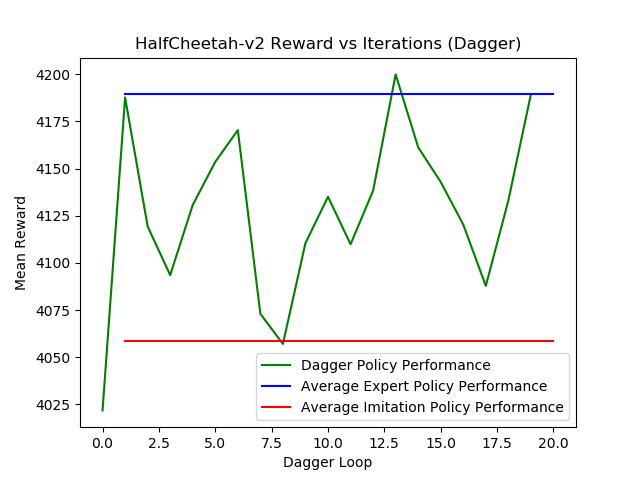
\includegraphics[scale=0.4]{HalfCheetah-v2Dagger}\\
    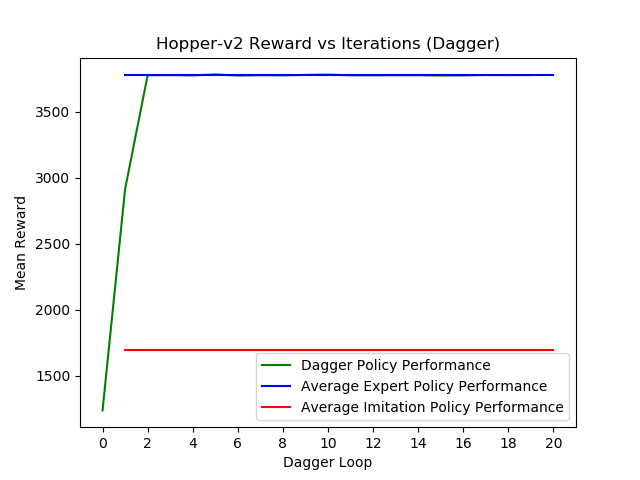
\includegraphics[scale=0.4]{Hopper-v2Dagger}
    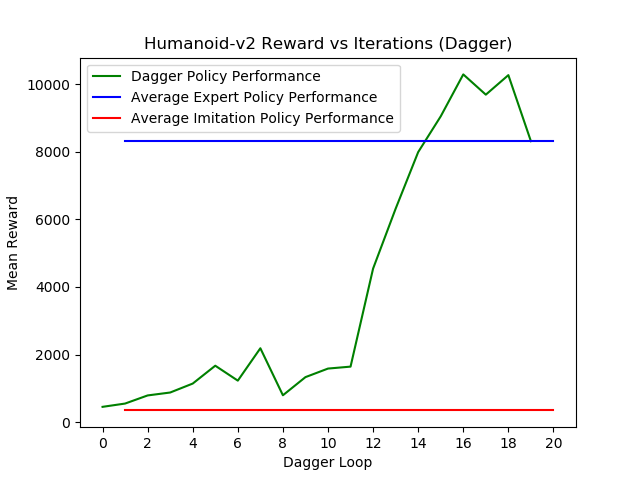
\includegraphics[scale=0.4]{Humanoid-v2Dagger}\\
    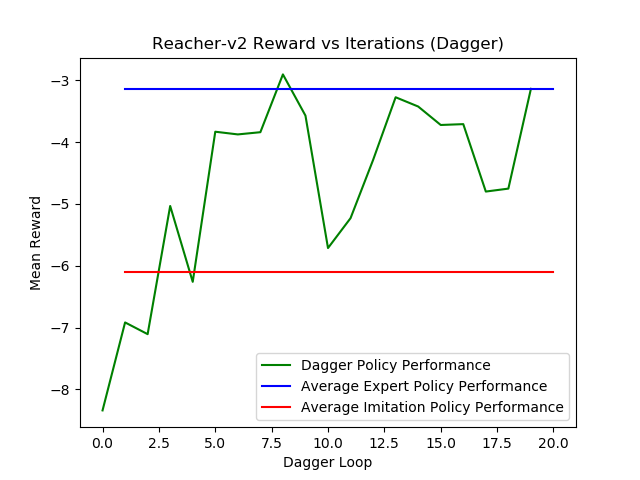
\includegraphics[scale=0.4]{Reacher-v2Dagger}
    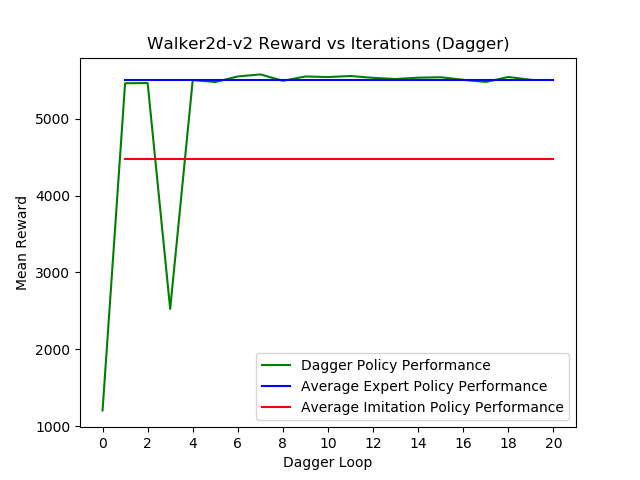
\includegraphics[scale=0.4]{Walker2d-v2Dagger}\\

\end{document}